%%%%%%%%%%%%%%%%%%%%%%%%%%%%%%%%%%%%%%%%%%%%%%%%%%%%%%%%%%%%%%%%%%%%%%%%%%%

\documentclass{standalone}

\usepackage{amsmath}
\usepackage{mathptmx}
\usepackage{pgfplots}
\usetikzlibrary{external}
\tikzexternalize{shortleaf-log}
\pgfplotsset{compat=1.16}

%% IEEE uses Times Roman font, so we'll default to Times.
%% These three commands make up the entire times.sty package.
\renewcommand{\rmdefault}{ptm}
\renewcommand{\ttdefault}{pcr}
\normalfont\selectfont

\begin{document}

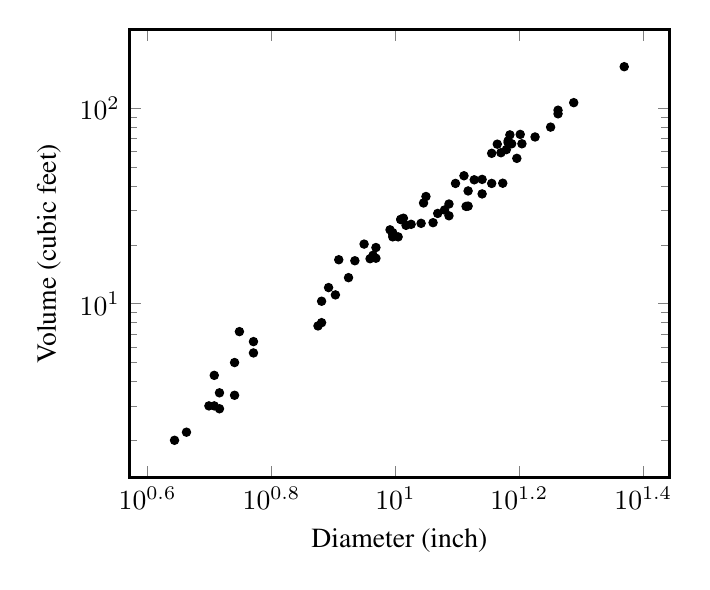
\begin{tikzpicture}
\tikzset{%%
  every mark/.append style={scale=1.0},%%
  scale=1.0%%
}
\pgfplotsset{%%
  every axis/.append style={font=\normalsize}%%
}
%%
\begin{loglogaxis}[%%
  axis line style=very thick,%%
  dotStyle/.style={mark size=1.5,black,mark color=black,mark=*,only marks},%%
  enlargelimits=true,%%
  %% x axis
  xlabel={\normalsize Diameter~(inch)},%%
  %% y axis
  ylabel={\normalsize Volume~(cubic feet)}%%
]
%%
%%
\addplot[dotStyle] coordinates {
  (4.4, 2)
  (4.6, 2.2)
  (5, 3)
  (5.1, 4.3)
  (5.1, 3)
  (5.2, 2.9)
  (5.2, 3.5)
  (5.5, 3.4)
  (5.5, 5)
  (5.6, 7.2)
  (5.9, 6.4)
  (5.9, 5.6)
  (7.5, 7.7)
  (7.6, 10.3)
  (7.6, 8)
  (7.8, 12.1)
  (8, 11.1)
  (8.1, 16.8)
  (8.4, 13.6)
  (8.6, 16.6)
  (8.9, 20.2)
  (9.1, 17)
  (9.2, 17.7)
  (9.3, 19.4)
  (9.3, 17.1)
  (9.8, 23.9)
  (9.9, 22)
  (9.9, 23.1)
  (9.9, 22.6)
  (10.1, 22)
  (10.2, 27)
  (10.2, 27)
  (10.3, 27.4)
  (10.4, 25.2)
  (10.6, 25.5)
  (11, 25.8)
  (11.1, 32.8)
  (11.2, 35.4)
  (11.5, 26)
  (11.7, 29)
  (12, 30.2)
  (12.2, 28.2)
  (12.2, 32.4)
  (12.5, 41.3)
  (12.9, 45.2)
  (13, 31.5)
  (13.1, 37.8)
  (13.1, 31.6)
  (13.4, 43.1)
  (13.8, 36.5)
  (13.8, 43.3)
  (14.3, 41.3)
  (14.3, 58.9)
  (14.6, 65.6)
  (14.8, 59.3)
  (14.9, 41.4)
  (15.1, 61.5)
  (15.2, 66.7)
  (15.2, 68.2)
  (15.3, 73.2)
  (15.4, 65.9)
  (15.7, 55.5)
  (15.9, 73.6)
  (16, 65.9)
  (16.8, 71.4)
  (17.8, 80.2)
  (18.3, 93.8)
  (18.3, 97.9)
  (19.4, 107)
  (23.4, 163.5)
};
\end{loglogaxis}
\end{tikzpicture}

\end{document}
